
%(BEGIN_QUESTION)
% Copyright 2012, Tony R. Kuphaldt, released under the Creative Commons Attribution License (v 1.0)
% This means you may do almost anything with this work of mine, so long as you give me proper credit

Calculate the amount of work done by this person pushing a lawnmower, given the force and displacement vectors shown:

$$\includegraphics[width=15.5cm]{i02616x01.eps}$$

\underbar{file i02616}
%(END_QUESTION)





%(BEGIN_ANSWER)

$$W = F x \cos \theta$$

$$W = (8 \hbox{ N}) (187 \hbox{ m}) \cos 28^o$$

$$W = 1320.9 \hbox{ N-m}$$

%(END_ANSWER)





%(BEGIN_NOTES)


%INDEX% Physics, energy, work, power

%(END_NOTES)


